% Latex File for The Progress Report
% Keywords cmd + F
% Page 1: TitleBookmark
% Page 2: AbstractBookmark
% Page 3: ContentsBookmark

\documentclass[a4paper]{article}

% Packages
\usepackage{hyperref}
\usepackage[a4paper, total={6.5in,10in}]{geometry}
\usepackage{multicol,caption}
\setlength{\columnsep}{1cm}
\usepackage{courier}
\usepackage{graphicx}
\newenvironment{Figure}
{\par\medskip\noindent\minipage{\linewidth}}
{\endminipage\par\medskip}
\usepackage[toc,page]{appendix}
\usepackage{etoolbox}
\usepackage{url}
\usepackage{hyperref}
\usepackage{csquotes}

% Code Package
\usepackage[utf8]{inputenc}
\usepackage{listings}
\usepackage{color}
\definecolor{codegreen}{rgb}{0,0.6,0}
\definecolor{codegray}{rgb}{0.5,0.5,0.5}
\definecolor{codepurple}{rgb}{0.58,0,0.82}
\definecolor{backcolour}{rgb}{0.95,0.95,0.92}
\definecolor{mygreen}{RGB}{28,172,0} % color values Red, Green, Blue
\definecolor{mylilas}{RGB}{170,55,241}
\lstdefinestyle{mystyle}{
	backgroundcolor=\color{backcolour},   
	commentstyle=\color{codegreen},
	keywordstyle=\color{magenta},
	numberstyle=\tiny\color{codegray},
	stringstyle=\color{codepurple},
	basicstyle=\footnotesize,
	breakatwhitespace=false,         
	breaklines=true,                 
	captionpos=b,                    
	keepspaces=true,                 
	numbers=left,                    
	numbersep=5pt,                  
	showspaces=false,                
	showstringspaces=false,
	showtabs=false,                  
	tabsize=2
}
\lstset{style=mystyle}
\setlength{\parindent}{0cm}
\patchcmd{\titlepage}
{\thispagestyle{empty}}
{\thispagestyle{plain}}
{}
{}

% MATLAB template
\lstset{language=Matlab,%
	%basicstyle=\color{red},
	breaklines=true,%
	morekeywords={matlab2tikz},
	keywordstyle=\color{blue},%
	morekeywords=[2]{1}, keywordstyle=[2]{\color{black}},
	identifierstyle=\color{black},%
	stringstyle=\color{mylilas},
	commentstyle=\color{mygreen},%
	showstringspaces=false,%without this there will be a symbol in the places where there is a space
	numbers=left,%
	numberstyle={\tiny \color{black}},% size of the numbers
	numbersep=9pt, % this defines how far the numbers are from the text
	emph=[1]{for,end,break},emphstyle=[1]\color{red}, %some words to emphasise
	%emph=[2]{word1,word2}, emphstyle=[2]{style},    
}


%------------------------------------------------------------------------------------------%
%-------------------------------DOCUMENT BEGINS--------------------------------------------%
%------------------------------------------------------------------------------------------%

\begin{document}
	
	% 1. TitleBookmark
	\begin{titlepage}
		\vspace*{\fill}
		\begin{center}
		\centering
		{\Huge Electronics and Computer Science \par}
		{\Huge Faculty of Physical Sciences and Engineering \par}
		{\Huge University of Southampton \par}
		\hfill \break
		{\Large Daniel Lee \par}
		{\Large \today \par}
		\hfill \break
		{\huge\bfseries Linear Quadratic Regulation using Reinforcement Learning \par}
		\hfill \break
		{\Large Project supervisor: Dr Bing Chu \par}
		{\Large Second examiner: Dr Mohammed El-Hajjar \par}
		\hfill \break
		{\large A progress report submitted for the award of \\
			\bfseries MEng Electronic Engineering with Artificial Intelligence \par}
		\end{center}
		\vspace*{\fill}
	\end{titlepage}
	\pagebreak
	\setcounter{page}{2}
	
	% 2. AbstractBookmark
	\section*{Abstract}
	The purpose of this project is to show the application of dynamic programming methods from \textit{Reinforcement Learning}, based on \textit{Bellman equation}, into discrete-time \textit{Linear Quadratic Regulation (LQR)} control theory systems. The progress that has been achieved so far includes the background reading of the core topics, numerical derivations of the Bellman equation, simulations on \textit{Greedy} and \textit{$\epsilon$-Greedy} algorithms and mathematical analysis of \textit{policy evaluation}, \textit{policy iteration} and \textit{policy improvement} in dynamic systems. Moreover, the \textit{Bellman Optimality Equation} for LQR systems was derived by solving the resulting \textit{Algebraic Riccati Equation}. FINISH LAST \par
	
	\pagebreak
	
	% 3. ContentsBookmark
	\tableofcontents
	
	\pagebreak
	
	\begin{multicols}{2}[
		\section*{Project description}
		FINISH LAST
		]
		
		\section{Background Research}
		With the purpose of getting familiar with the core topics of this project, a great portion of the available time was invested in reading the appropriate literature. For the topic of reinforcement learning, the main source of reference was the book titled \enquote*{\textit{Reinforcement Learning: An Introduction}} by Sutton and Barto \cite{reinfbook}. With respect to Linear Quadratic Regulation, the research was mainly based on the article \enquote*{\textit{Reinforcement Learning and Feedback Control}} by Lewis, Vrabie and Vamvoudakis \cite{lqrart}.\par
		
		\section{Reinforcement Learning}
		The concept of reinforcement learning describes the computational process that an agent executes when interacting with the given environment. It provides the \textit{agent} with mathematical algorithms to maximize the long-term return by taking optimal decisions from a set of states and actions that belong to the given \textit{environment}.\par
		
		\subsection{System Elements}
		The reinforcement learning system is composed of three main elements: \enquote{a \textit{policy}, a \textit{reward} and a \textit{value}} \cite{reinfel}. A policy maps the actions that the agent should select to the states of the environment. In simpler words, it determines the way in which the agent should behave in different situations. When an agent selects an action from a state, it collects a numerical value called reward. A reward quantitatively expresses how positive the performance of the action taken at a state was. While a reward represents an immediate acquisition, the \textit{value} of a state provides the information of the total expected reward, or \textit{return}, of the state or state-action pair. Therefore, it can be considered as a quantity that expresses how much the agent can benefit in the long-term.\par
		
		\subsection{K-arm Bandit Problem}
		A good example that illustrates these concepts in practice is the \textit{k-arm bandit problem}. In this scenario, the aim of the agent is to maximize its return by pulling the desired arm, among the k number of arms, from the bandit, at each finite discrete step, or turn. To solve this problem, two simple methods can be implemented. These are the \textit{greedy} method and the \textit{$\epsilon$-greedy} method. \par
		
		\subsubsection{Greedy Method}
		The greedy method represents a policy where the agent always chooses the action that has the highest expected reward. In the case of the k-arm bandit problem, the expected reward of an action, or \textit{value} $Q_t(a)$, can be expressed with equation (1), where $a \in A$ and $k$ represents the number of times that the actions was selected before the current time $t$. \par
		
		\begin{equation}
			Q_t(a) = \frac{R_1 + R_2 + ... + R_{K_a}}{K_a}
		\end{equation}
		
		The equation shows that every time the action, or arm, is selected by the agent, its value is updated by averaging all the past collected rewards. This means that if an action was selected an infinite amount of times, $k\to\infty$, its value would eventually converge to its \textit{actual} value $Q_*(a)$. Therefore, at every turn, the agent will pull the arm that returned the most profit in past experiences. This can be represented by (2). \par
		
		\begin{equation}
			Q_t(A_t^*) = max_a Q_t(a)
		\end{equation}
		
		However, as in many real cases, the bandit problem is a stochastic system where the immediate reward has a probability distribution, or noise, that might negatively affect the agent's short-sighted decisions. An agent could be ignoring the optimal action only based on few past experiences and never come back to it again. To further demonstrate this, a simulation of this example was performed by creating a MATLAB function called \textit{greedy}, Appendix A. The greedy function's inputs are, the number of bandits, the number of actions, the number of turns, the Gaussian distribution parameters to set the actual action values and the Gaussian distribution parameters to set the noise for every immediate reward. For this simulation, the initial actual values $Q_*(a)$ for all $a \in A$ were selected from a set of numbers from a Gaussian distribution $\mathcal{N}(0,1)$. In addition to this, Gaussian noise $\mathcal{N}(0,3)$ was added to all immediate rewards $r \in R$. For a more accurate evaluation, the results for the 15-arm bandit problem were averaged over 1000 bandits. Figure 1 illustrates how often the agent converged to the optimal action $a^*$, over a 1000 steps. \par
		
		\begin{Figure}
			\centering
			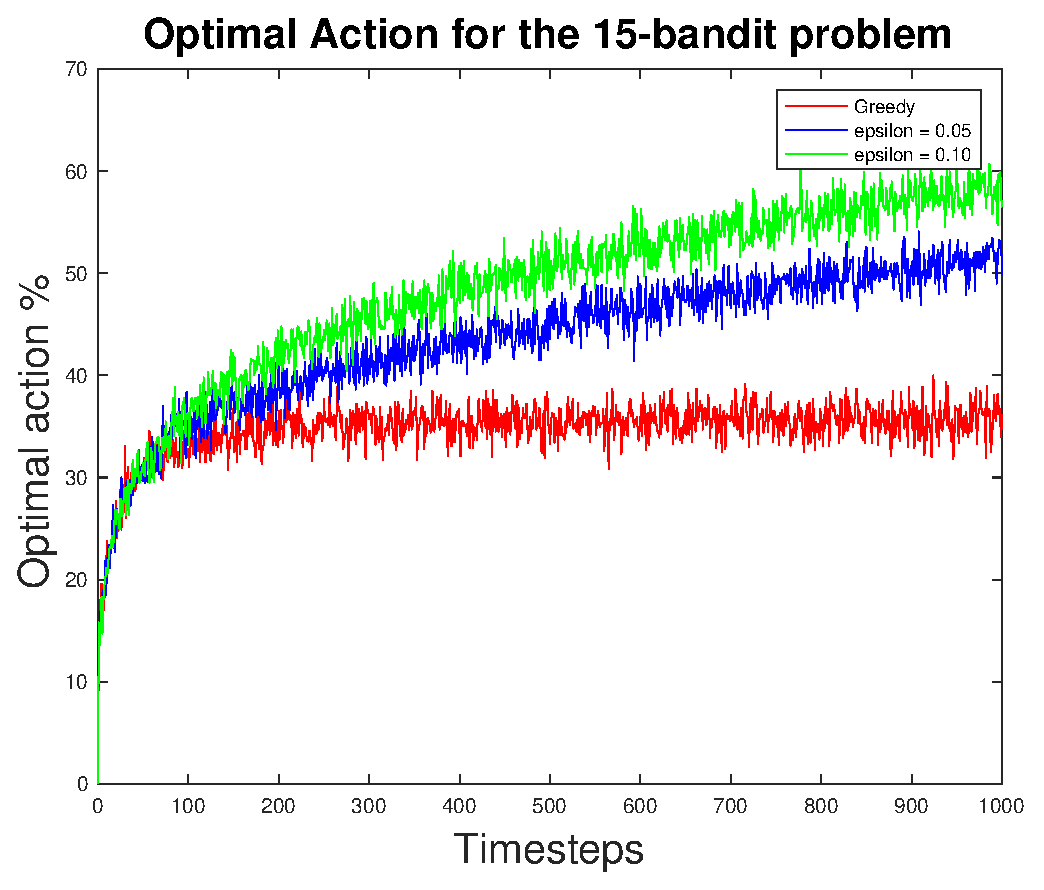
\includegraphics[width=\linewidth]{allplot2.eps}
			\captionof{figure}{Optimal action percentage}
		\end{Figure}
		
		From the graph above, it can be seen that greedy algorithm led the agent to converge to the optimal action in around $\%35$ of the cases. To improve the performance of the agent in the long term, it is possible to use a slight variation of this method called the \textit{$\epsilon$-Greedy} method. \par
		
		\subsubsection{-Greedy}
		
		From the previous subsection, the theory and implementation of the greedy algorithm were shown. In this section, a variation of the greedy algorithm called $\epsilon$-Greedy will be explored. One of the issues from the $\epsilon$-Greedy was that because it always forced the agent to choose the best action-value in every state, if a particular action-value was low from the start, the agent never chose it for the rest of the simulation, therefore, never being able to discover its \textit{actual} value. To avoid this problem, a variant of this algorithm that allows the agent to \textit{explore} from time to time can be used. In every state, the agent will randomly choose an action with equal probability in all of them. This means that because if an action is chosen infinite times it converges to its textit{actual} value, this will allow the agent to have a more precise information of its options. This algorithm is called $\epsilon$-Greedy.
		
		The first simulation was created by using an $\epsilon$ of 0.1. The 5-bandit problem was run for 600 steps and averaged over 300 tasks. The result was then compared to the optimal return. This can be seen in the figure below.
	
		\begin{Figure}
			\centering
			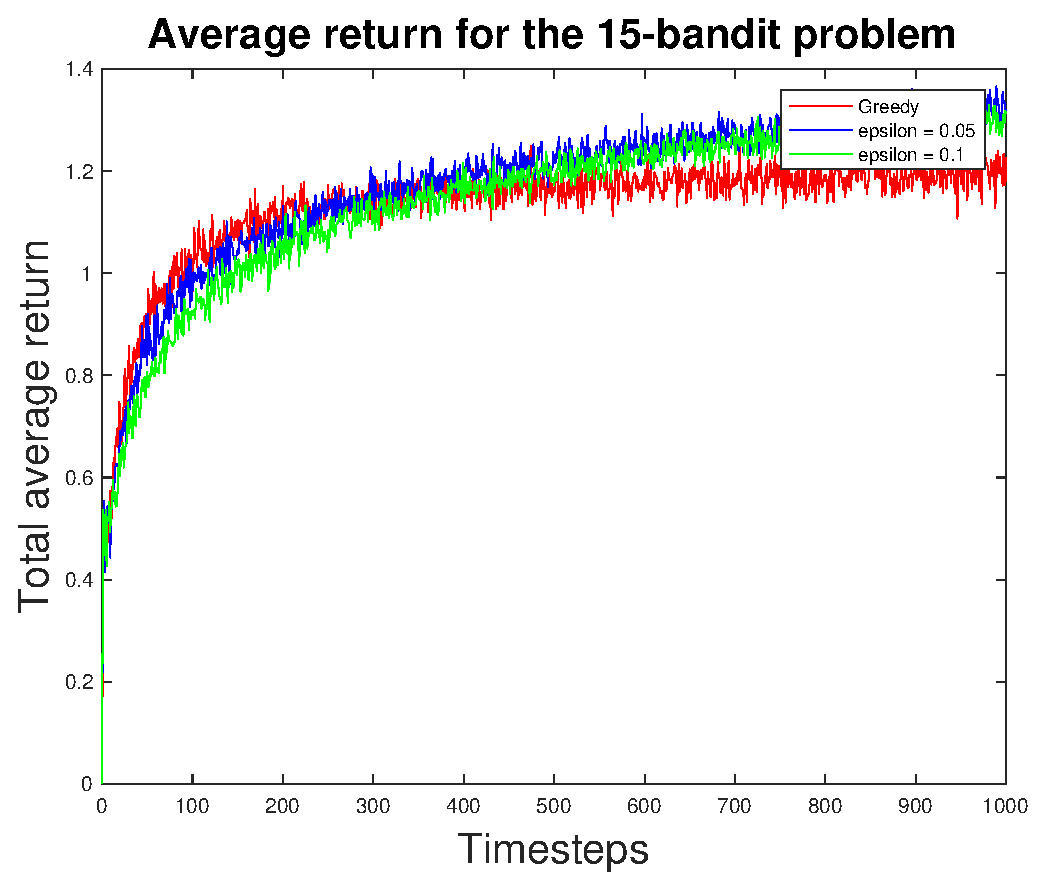
\includegraphics[width=\linewidth]{allplots1.eps}
			\captionof{figure}{Optimal action percentage}
		\end{Figure}
		
		From the graph above, we can see that opposed to the greedy algorithm, the average reward gets closer to the optimal average reward as the number of steps increases. In theory, as the number of steps goes to infinity, the average reward would converge to the optimal reward. 
		
		Following this, a plot showing the percentage in which the agent converged to choose the optimal value is shown below.
		

		
		From analyzing the graph above, we can see that as we reach step 600, the optimal action percentage reaches around 90 percent. This is because we allow the agent to explore for 10 percent of the time. This means that although 10 percent of the time the action might not receive the maximum immediate reward, it will aid the agent to get a more precise estimate of the real value. 
		
		For the last e-greedy simulation, an epsilon value of 0.01 was used. The first simulation compares the average return of this particular e-greedy algorithm against the optimal return.
		
		
		From this graph, we can see that the average return increases steadily. If the number of steps is increased, this version of the e-greedy algorithm will outperform the other ones and eventually converge to an accuracy of optimal action to 99.9 percent.
		
	
		A more helpful graph is plotted above and show how how the optimal action percentage is steadily increased. Although is not as fast as using an epsilon 0.1, again, in the long run this configuration will outperform the previous configuration.
		
		\section{Dynamic Programming}
		\subsection{Policy Evaluation}
		The idea behind policy evaluation is to find the state-value for all the possible states using an arbitrary policy $\pi$. To compute the state-value we use one of Bellman's equations:
		
		\begin{equation}
			v_{k+1}(s) = \mathbf{E}_\pi[R_{t+1} + \gamma v_k(S_{t+1}) | S_t = s]
		\end{equation}
		
		This equation computes the estimated state-value for the following time step using information from the current state. This method is called full back up, because it uses the information in the values of all the available states to estimate a state-value.
		
		\subsection{Policy Iteration}
		In order to converge to the $v_\pi$ of each state we can iterate over the episodic system many times. This concept is called \textit{policy iteration}.
		
		\subsubsection{Gridworld example}
		Policy iteration can be applied in the gridworld scenario. \cite{Woer}
		
		
		
		
		\end{multicols}
		\newpage
	
		% Start of APPENDIX
%		\begin{appendices}
%		\chapter{Greedy function MATLAB code}
%			\lstinputlisting{greedy.m}
%		\chapter{e-Greedy function MATLAB code}
%			\lstinputlisting{egreedy.m}
%		\end{appendices}



\bibliographystyle{ieeetr}

\bibliography{biblio}

\end{document}











